\chapter{The Edge of the Model}
\label{ch:model-boundary}

A0 and the two scalar slices make many program claims precise. They do not
contain every state that a modern processor exposes or every behavior that
software can observe. The boundary is not a miscellaneous list of hard
problems. Each item in this chapter identifies structure absent from the model
we built.

That way of organizing omissions matters. ``The model does not support
floating point'' sounds like a missing feature checkbox. ``The state has no
rounding mode, floating-point exceptions, or representation for NaN'' names
what a definition must add. One description invites a larger instruction
table. The other begins a semantic design.

\begin{keyidea}[title={Every boundary names missing state or missing observation}]
When a claim falls outside the scalar model, ask what new state can affect the
movement and what new observation can distinguish outcomes. Extend those
definitions before extending the proof machinery.
\end{keyidea}

\section{A model is an instrument, not a miniature universe}

A scientific model is built for questions. A map that shows streets may omit
soil composition; a geological map may omit turn restrictions. Neither is
false merely because it cannot answer the other's question. It becomes
misleading when its user forgets the purpose of the abstraction or treats an
omitted distinction as an established equality.

Our scalar architectural model answers questions about decoded instructions,
word and memory effects, control transfer, normal and trapped outcomes,
selected calling conventions, and observations over those states. It can
support a theorem that three loops return the same XOR reduction. It cannot,
without extension, support a theorem that they consume the same energy, reveal
the same information through a cache, behave alike under another thread's
writes, or survive a page-table change.

The recurring error is to ask a strong question of a weak observation. If
timing is absent, every timing difference is invisible. If speculative state
is absent, a proof cannot constrain speculative accesses. If the program map
is immutable, a theorem cannot describe a store that changes future decoded
instructions. Silence in the model is not evidence of absence in the machine.

\begin{figure}[htbp]
\centering
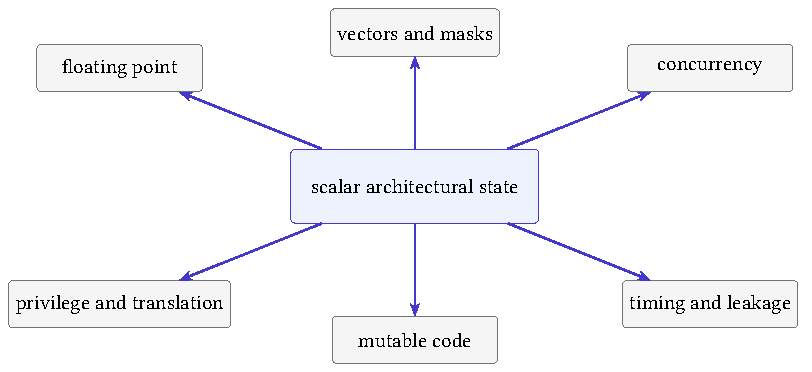
\includegraphics[width=0.94\textwidth]{figures/model-boundary-map}
\caption{The scalar architectural core is surrounded by extensions, each of
which adds state, transitions, observations, or all three.}
\figalt{A central box for scalar architectural state connects outward to floating point, vectors, concurrency, privilege, mutable code, leakage, and compilation.}
\label{fig:model-boundary-map}
\end{figure}

\begin{definition}[title={Honest model extension}]
An extension states the new values and state components, defines how
transitions read and write them, enlarges observations only as required, and
revisits every preservation or refinement theorem whose premises mention the
old state. It also supplies a conservative-embedding argument when old programs
are expected to retain their old meaning.
\label{def:honest-model-extension}
\end{definition}

The final clause protects earlier work. Adding vector registers should not
quietly change scalar addition. Adding virtual memory should explain when the
old flat-address model embeds into the new model, perhaps under an identity
translation and stable permissions. The extension may reveal that an earlier
claim needed a stronger premise. That is a correction, not a failure of the
method.

\section{Floating point adds an arithmetic environment}

An integer word represents one residue modulo a power of two, with optional
signed and unsigned readings. A floating-point datum has a different
structure: sign, significand, exponent, finite and infinite values, signed
zero, and values that represent ``not a number.'' Operations depend on a
destination format and a rounding direction. They may also report exception
conditions. IEEE 754 specifies formats, operations, exception conditions, and
default handling for binary and decimal arithmetic
\autocite{ieee7542019}.

The familiar algebraic laws need review. Floating-point addition is generally
not associative because intermediate rounding depends on grouping. Two
mathematical expressions that are equal over real numbers may produce
different floating-point values. NaN comparisons do not behave like an
ordinary total order. Positive and negative zero compare equal in selected
operations while retaining distinguishable encodings and behavior elsewhere.

\begin{example}[title={A regrouping can change a result}]
Choose a format and finite values where adding a small \(y\) to a large \(x\)
rounds back to \(x\), but adding \(y\) to \(-x\) first leaves a representable
small result. Then \((x+y)+(-x)\) can differ from
\(x+(y+(-x))\). A proof that rewrites by real-number associativity would be
invalid for that floating-point operation.
\end{example}

An A0 floating-point extension would need floating registers or a declared
reuse of integer registers, supported formats, operation semantics, rounding
state, exception flags, and conversion rules. The observation must say whether
it compares exact encodings, numerical classes, exception state, or some
combination. A solver route needs floating-point theories or a sound reduction
to bit vectors; a certificate route must cover whichever semantics it uses.

\begin{warning}[title={Bit-pattern equality and numerical agreement differ}]
Two floating-point results may be numerically interchangeable for one client
yet have different zero signs, NaN payloads, or exception histories. State the
observation before calling an optimization correct.
\end{warning}

\section{Vectors add shape, masks, and partial activity}

A packed or vector instruction does not merely apply a scalar operation to a
wider word. It introduces lanes, element widths, lane ordering, masks, tail
policy, and wider register state. Scalable vector designs may make the active
length a state-dependent quantity rather than a constant in the program text.
Loads and stores add stride, grouping, fault, and partial-completion questions.

Chapter 15's XOR reduction suggests the appeal. Several words can be loaded
and combined in parallel, then the lanes can be reduced to one word. The
correctness proof needs a partition of the input region, a mapping from memory
indices to lanes, an invariant for partial lane accumulators, and a final
horizontal reduction lemma. A tail whose length is not a multiple of the
vector width needs masking or a scalar remainder path.

\begin{figure}[htbp]
\centering
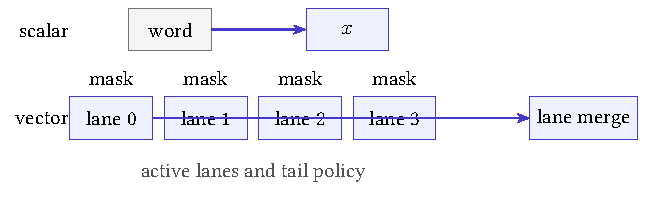
\includegraphics[width=0.92\textwidth]{figures/scalar-vector-extension}
\caption{A scalar reduction carries one accumulator. A vector reduction adds
lane state, an activity mask, a tail policy, and a final lane merge.}
\figalt{The scalar path shows one word at a time entering x; the vector path shows four lanes under a mask entering four accumulators and then one merge.}
\label{fig:scalar-vector-extension}
\end{figure}

The existing scalar proof is still useful. It supplies the specification and
the algebraic XOR laws. It does not supply lane semantics or the partition
proof. Optional vector extensions belong here rather than at the book's center
because the scalar core is the shared foundation for both RISC and CISC
architectures; a particular vector extension is one elaboration of that core.

An honest Axeyum vector package should begin with a small lane model and
controls for inactive lanes, tail elements, lane order, and masked faults. Old
archived shuffle or bit-manipulation artifacts may inform tests, but they do
not define the new package's semantics or establish its claims.

\section{Concurrency replaces one trace with an event structure}

The book's executions are single-threaded sequences. At each step one
instruction reads one state and produces one successor. With multiple agents,
memory actions can overlap in time, observations can depend on ordering, and a
global sequence may be too strong or too weak a description.

Lamport's formulation of sequential consistency asks for results equivalent
to one sequential order that preserves each processor's program order
\autocite{lamport1979multiprocessor}. Modern weak-memory models permit selected
reorderings while constraining them through relations such as program order,
reads-from, coherence, and synchronization. The object of study becomes a set
or graph of events plus consistency conditions.

Consider two threads that each write one location and read the other. A
single-thread proof can establish each thread's local instruction effects. It
cannot determine which paired read results the whole system permits. That
question needs shared-memory events, an architectural memory model, and an
observation containing both threads' outcomes.

\begin{figure}[htbp]
\centering
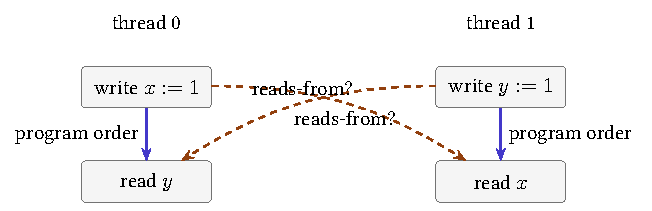
\includegraphics[width=0.86\textwidth]{figures/trace-to-event-graph}
\caption{Concurrency adds relations across local traces. Program order alone
does not determine reads-from or the allowed global observation.}
\figalt{Two vertical thread traces contain read and write events; horizontal arrows connect a write in one thread to a read in the other.}
\label{fig:trace-to-event-graph}
\end{figure}

Atomics add indivisibility and ordering contracts. Fences constrain event
relations. Read-modify-write operations combine a read and conditional write
under special rules. A state extension with merely two program counters is
therefore insufficient; it would still lack the memory-event semantics that
make the extra execution meaningful.

The proof style changes as well. Invariants may describe shared resources and
interference. Refinement may compare sets of allowed executions rather than
one successor at a time. A counterexample is an event graph with a forbidden
or surprising outcome, and replay means validating every event and relation
against the memory model.

\section{Privilege and virtual memory put addresses in context}

Our scalar memory maps addresses directly to bytes and checks whether a range
exists. An operating system and privileged architecture add translation,
permissions, modes, exceptions, and control registers. A virtual address may
name different physical storage in different address spaces. The same address
may be readable, executable, or forbidden depending on privilege and page
attributes.

Address translation is itself a movement through state. Page-table entries are
read, permissions are checked, and translation caches may retain derived
information. A load theorem that begins with ``effective address \(a\)'' no
longer reaches memory directly. It needs a translation result or fault. An
instruction fetch and a data load may use related but differently constrained
translation paths.

The smallest clean extension can treat translation as an abstract function of
virtual address, access kind, and privileged state. A deeper model can expose
page walks and translation caches. The right choice depends on the theorem.
A user-level functional proof may assume a stable valid mapping. A page-table
update proof cannot hide the walk. A side-channel proof may need translation-
cache observations that both functional models omit.

\begin{definition}[title={Contextual address meaning}]
In a translated machine, an address does not identify storage by itself. Its
meaning depends at least on the address space, access kind, privilege state,
translation structures, and permission policy selected by the model.
\end{definition}

Interrupts and exceptions add another control source. The next instruction may
not be the architectural successor of the current user instruction; execution
may enter a handler with saved state. Returning from that handler has its own
privilege and restoration rules. A proof that assumes uninterrupted procedure
execution must state that premise or model the interference.

\section{Self-modifying code joins program and data memory}

A0 deliberately keeps an immutable program map separate from mutable data
memory. That design makes decoding stable: the instruction at a program
counter cannot change because of an ordinary store. Real systems can generate,
load, patch, or overwrite code. Once data writes can affect future fetches, the
program is part of evolving state.

The naive extension is to use one byte map for both fetch and data access. That
is necessary but not always sufficient. Instruction and data views may require
architectural synchronization before new bytes are guaranteed to be fetched.
Decoders with variable-length instructions may see changed boundaries. Another
thread may race with the modification. Permissions may prohibit simultaneous
write and execute access to a page.

\begin{example}[title={A store can invalidate the next proof step}]
Suppose a proof decodes the instruction at address \(p\), then reasons about a
store, then applies the saved decoded instruction at \(p\). If the store can
alter bytes in that instruction, the proof has reused stale syntax. It must
show that the written range is disjoint from the fetched range or perform the
architecture's required synchronization and decode again.
\end{example}

This boundary reaches ordinary tooling. Linkers relocate instructions and
loaders place segments before execution begins. Just-in-time compilers create
new code while a process runs. Dynamic patching changes code already in use.
Each activity needs a phase or transition model that binds bytes to the moment
at which their semantics is claimed.

An Axeyum extension should therefore make decode results depend on a code-memory
version or digest. A negative control can modify one instruction byte after a
cached decode and require the stale step to be rejected. Another can omit a
required synchronization event and require the execution route to refuse the
stronger claim.

\section{Timing and leakage require richer observations}

Two programs can be functionally equivalent and still take different time,
touch different cache sets, contend for different resources, or draw different
power. The scalar model projects all of those distinctions away. It cannot
establish constant-time behavior because it contains neither a time measure
nor the events through which time varies.

The Spectre work demonstrated that speculative execution can affect
microarchitectural state and reveal information even when architectural
control later discards the speculative path \autocite{kocher2019spectre}.
A purely architectural trace can show that the discarded instructions wrote
no committed register or memory value. That fact does not describe their cache
effects or the time needed by a later probe.

\begin{figure}[htbp]
\centering
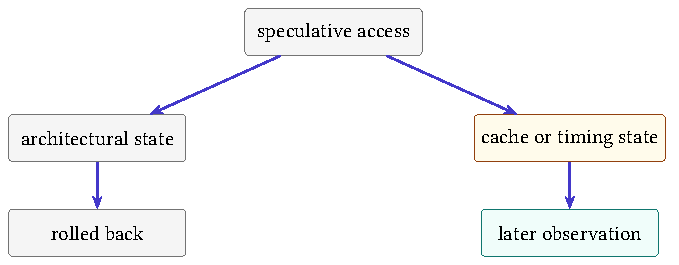
\includegraphics[width=0.88\textwidth]{figures/architectural-leakage-split}
\caption{Architectural rollback can erase committed effects while a richer
observation retains timing or cache consequences.}
\figalt{A speculative branch splits into a discarded architectural path and a surviving microarchitectural observation measured by a later probe.}
\label{fig:architectural-leakage-split}
\end{figure}

A constant-time model might record an abstract leakage trace containing branch
directions and memory addresses while omitting actual cycle counts. A cache
model might record sets, tags, replacement state, and hits. A contention model
might add execution ports or shared queues. A power model needs a different
abstraction again. There is no single side-channel state that answers every
leakage question.

\begin{warning}[title={Functional equivalence is not a security theorem}]
Equal architectural outputs under equal public inputs do not imply equal
timing, equal memory-access patterns, or equal speculative effects. A security
claim must name secrets, public observations, attacker capabilities, and the
leakage model.
\end{warning}

The proof relation also changes. A \keyterm{noninterference} statement compares
two runs that differ in secret data and
requires their public observations to agree. Negative controls should change a
secret-dependent address or branch and require the leakage checker to notice.
A result-only checker would accept the mutation and thereby expose its own
inadequate observation.

\section{Verified compilation adds a tower of languages}

Our cross-ISA proofs begin with machine programs on both sides. A compiler
starts higher: source syntax, types, undefined or unspecified behavior,
intermediate representations, optimization passes, assembly, object files,
linking, loading, and target execution. Each level has states and observations,
and each translation needs a preservation statement.

CompCert showed that a realistic compiler could be developed with a proof of
semantic preservation from a substantial C-like source language to assembly
\autocite{leroy2009compcert}. Its importance here is methodological. The
theorem does not say ``the compiler is correct'' without qualification. It
names source and target semantics and a relation between their behaviors.

Undefined source behavior is a sharp boundary. If a source execution has no
promised meaning after an invalid operation, a target behavior need not refine
a result the source never specified. Conversely, machine details such as finite
memory or resource exhaustion may introduce target outcomes that a source
model must accommodate. The exact direction and premises of refinement matter.

Separate compilation adds interfaces between units. Linking adds symbol
resolution and relocation. Loading adds addresses, permissions, and initial
machine state. A verified compiler theorem cannot by itself establish a claim
about a final executable if tools outside the proof or unchecked assumptions
break the chain.
The evidence manifest must bind the whole route actually used.

\begin{figure}[htbp]
\centering
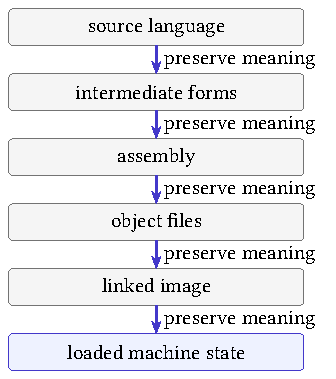
\includegraphics[width=0.92\textwidth]{figures/compilation-tower}
\caption{A source-to-machine claim crosses several semantic interfaces. Each
arrow needs a preservation theorem or an explicitly trusted boundary.}
\figalt{A vertical tower runs from source through intermediate forms, assembly, object, linked image, and loaded machine state, with labeled refinement arrows.}
\label{fig:compilation-tower}
\end{figure}

Axeyum can contribute solvers, certificates, and kernel reconstruction to
local obligations in such a tower. It does not currently provide this book
with a verified source language, compiler, linker, loader, and complete
real-machine semantics. The right introductory path is to verify one small
translation pass or one instruction-selection rule, then compose only after
the interfaces and controls are stable.

\section{How to extend the workbench without blurring it}

Every extension should pass four gates. The \keyterm{state gate} inventories
new components and preservation rules. The \keyterm{step gate} defines legal
transitions and failure classes. The \keyterm{observation gate} states which
new distinctions the theorem exposes. The \keyterm{evidence gate} binds
executors, formulas, certificates, and controls to those definitions.

\begin{figure}[htbp]
\centering
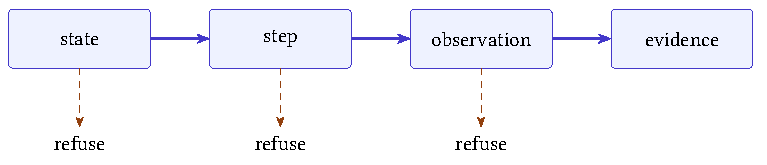
\includegraphics[width=0.9\textwidth]{figures/extension-gates}
\caption{An extension reaches evidence only after state, transition, and
observation contracts are explicit.}
\figalt{Four gates in order are labeled state, step, observation, and evidence; unsupported inputs leave through refusal arrows.}
\label{fig:extension-gates}
\end{figure}

Start with a conservative miniature. A floating-point lesson might support one
format, one rounding mode, and addition, while rejecting every other form. A
concurrency lesson might support two threads and a tiny event language. A
virtual-memory lesson might use one-level translation. Small scope is honest
when unsupported cases are visible refusals rather than silent defaults.

The Rust layer should own the typed semantic core and evidence-critical
checking. Python should construct examples, call that core, display traces,
and help readers mutate controls. This repeats Chapter 15's division. As the
model grows, a single implementation boundary becomes more valuable, not less.

Machine evidence cannot replace the conservative-extension argument. Before
reusing an old scalar theorem, show that executing an old instruction from an
embedded old state produces the embedded old successor and does not touch new
state in an observable way. A counterexample to that property identifies an
interaction that the extension must expose.

\begin{proofkit}[title={Template for a conservative extension}]
Let \(E\) embed old states into new states, \(s\) be an old legal state, and
\(I\) an old instruction. Show that the new decoder recognizes the same
instruction and that one new step from \(E(s)\) reaches \(E(s')\) exactly when
the old step from \(s\) reaches \(s'\). State separately how new components are
initialized and preserved. Then prove that the new observation of \(E(s)\)
agrees with the old observation of \(s\).
\end{proofkit}

\section{Three ways boundary claims go wrong}

The first failure is \keyterm{silent completion}: an unsupported case is given
a convenient default. A floating-point decoder treats an unknown format as
binary64. A vector checker treats absent mask semantics as ``all lanes active.''
A memory model orders events that it does not know how to relate. The tool
returns an answer, but the answer belongs to an invented model.

The repair is refusal. Unsupported instructions, formats, privilege modes,
events, and observations must have typed failure outcomes. A report can then
distinguish ``the claim is false'' from ``this semantic route does not cover
the claim.'' That distinction is as important at the model edge as it was for
solver evidence in Chapter 14.

The second failure is \keyterm{decorative state}. New fields appear in a state
record but no transition reads or writes them. Adding a rounding-mode field
does not create floating-point semantics if every operation still uses one
hard-coded rounding rule. Adding a cache map does not create a leakage model if
speculative and committed accesses never update it. State earns its place by
participating in defined movements and observations.

The third failure is \keyterm{accidental theorem transport}. An earlier proof
is reused because the old syntax still parses. Yet a new transition may change
an old instruction's effect, a new observation may reveal an old hidden write,
or a new context may distinguish programs that were interchangeable before.
Conservative embedding must be established; textual inclusion is not enough.

\begin{table}[htbp]
\centering
\caption{Typical boundary mistakes and controls that expose them.}
\begin{tabular}{@{}p{0.25\textwidth}p{0.31\textwidth}p{0.34\textwidth}@{}}
\toprule
Mistake & Hidden assumption & Negative control \\
\midrule
Silent completion & unknown means default & supply one unsupported form \\
Decorative state & new field cannot matter & vary it while holding old state fixed \\
Accidental transport & old theorem survives automatically & expose a new observation or context \\
Layer collapse & one checker covers every layer & mutate the unbound translation step \\
\bottomrule
\end{tabular}
\end{table}

A fourth failure, layer collapse, appears when one successful check is allowed
to stand for several missing connections. A verified event-graph checker does
not show that machine bytes generated that graph. A floating-point solver does
not show that an instruction decoder selected the intended format. A compiler
proof does not verify an unmodeled loader. The claim-to-evidence chain grows as
the model grows; no link becomes optional because another link is strong.

\section{A research question for every new component}

Adding state should immediately produce proof questions. For each new component
\(q\), ask how it is initialized, which transitions can read it, which can
write it, and which transitions must preserve it. Ask whether it affects
legality or only results. Ask whether the observation exposes it directly or
through later behavior. Finally ask how a malformed or adversarial value of
\(q\) reaches a refusal.

For floating point, \(q\) might be the rounding mode. Initialization selects
a mode; arithmetic reads it; a control-register write may change it; integer
addition preserves it. The result observation may reveal it only indirectly
through rounded values, while a full-state observation sees it directly. A
control changes the mode on a halfway case and requires a changed result.

For concurrency, the new object may be a reads-from relation rather than a
register field. Its endpoints must be compatible read and write events, values
must agree, and the whole graph must meet the architectural consistency rules.
A control redirects one read to an incompatible write and requires rejection.
This shows why ``state component'' should be read broadly: event relations and
histories can be semantic state even when no hardware register stores them.

For leakage, the component might be an address trace. Every selected load and
store appends an address; non-memory instructions preserve the trace; the
security observation projects it. A control changes a secret-dependent index
while preserving the final architectural result. The functional checker still
accepts, but the leakage comparison must reject.

\begin{tryit}[title={Write the five questions before the semantics}]
Choose a boundary component and answer: how is it initialized, who reads it,
who writes it, who preserves it, and which observation can distinguish it?
Then design one unsupported input and one semantic mutation for the checker.
\end{tryit}

This worksheet prevents feature lists from outrunning definitions. It also
creates the first test plan. Each answer suggests a positive path, a
preservation check, and a negative control. When no observation can distinguish
the new state, ask whether the theorem truly needs it or whether its effect is
only latent in a larger context.

\section{An Axeyum learning sequence beyond the scalar core}

The next Axeyum lessons should grow one semantic dimension at a time. A useful
sequence is: one binary floating-point addition with a fixed format; the same
operation under two rounding modes; a four-lane integer operation with a mask;
two single-event threads under sequential consistency; then one permitted
weak-memory outcome. Each lesson adds one state idea and one checker attack.

The Rust package for a lesson should expose constructors that make unsupported
cases impossible or explicit. The Python layer should show the state before
and after a step, run a positive miniature, fire a named mutation, and print
the trust boundary. Only after the miniature is stable should symbolic inputs
and solver routes be added.

Kernel reconstruction belongs last in this sequence, not because it is
unimportant, but because it can only reconstruct the proposition it receives.
First bind bytes or events to semantics. Then validate the semantic relation.
Then translate a bounded obligation and check its certificate. A kernel proof
over an unbound formula would certify the wrong layer with great confidence.

\section{Choosing the next boundary}

The most attractive extension is not always the best next one. Choose a claim
whose missing state is small enough to define completely, whose official
sources can be pinned, whose examples fit in a reader trace, and whose controls
can fail for recognizable reasons. A fashionable topic with an ambiguous
semantic boundary will produce impressive artifacts and weak conclusions.

For this book's workbench, a narrow floating-point operation or a two-thread
memory litmus test would be plausible next lessons after the scalar packages
exist. A full speculative out-of-order processor or verified optimizing
compiler would be a different project. The distinction is one of semantic
surface, not ambition.

There is also a maintenance test. A good extension makes its new state visible
in definitions, traces, observations, serialization, and controls. If adding
one rounding mode or mask bit requires unexplained special cases throughout
the old scalar executor, the boundary has not been isolated cleanly. The
design should let old scalar claims retain their former meaning while new
claims opt into the richer state.

The scalar core remains valuable at every edge. Words still encode fields.
States still need inventories. Instructions still produce movements. Proofs
still depend on observations. Counterexamples still need replay. Evidence still
needs a claim, a checker, and a control. The universal method is not one
instruction set; it is the discipline of naming meaning before trusting
agreement.

The boundary is therefore an invitation, not an apology. Each omitted concept
opens a new version of the book's central mystery: how a finite inscription can
govern a movement, how different inscriptions can share meaning, and how a
checker can know. The answers become harder as state grows, but they remain
approachable when the new distinctions are named one at a time. Precision does
not drain the wonder from computation. It lets us see exactly where the wonder
has moved.

\section{Exercises}

\begin{enumerate}
\item \textbf{Execute.} Choose one floating-point format and classify positive
zero, negative zero, infinity, and one NaN by their fields.
\item Give a concrete finite floating-point example in which reassociating
three additions changes the result. Name the rounding mode.
\item Define an observation that treats all NaNs alike and another that compares
their encodings. Give a pair the two observations classify differently.
\item \textbf{Break.} Add vector lanes but omit the activity mask from state.
Construct two executions that the incomplete model confuses.
\item State a loop invariant for a four-lane XOR reduction with a masked tail.
Name the partition represented by each lane.
\item Explain why a scalar proof of XOR associativity is useful but insufficient
for a vector memory-access proof.
\item Draw the events for the two-thread store-and-load example. Add program-
order and two possible reads-from relations.
\item State Lamport's sequential-consistency condition in your own words. Which
part cannot be expressed by two unrelated local traces?
\item Design a negative control that removes one fence from a concurrent
program and changes an allowed observation.
\item Add an abstract address-translation function to A0. List its inputs and
its success and fault outcomes.
\item Give premises under which flat A0 memory embeds into that translated
model as an identity mapping.
\item \textbf{Break.} Allow a store to change program bytes while retaining a
cached decode. Give the shortest stale-instruction trace you can.
\item Define a code-memory version check that would reject the stale trace.
\item Give two programs with equal return values and different address traces.
Explain why result equivalence does not establish constant-time behavior.
\item Define public and secret inputs for a two-run noninterference claim. State
the observation that must agree.
\item Add a speculative cache event to one path and roll back architectural
state. Which observation detects the remaining difference?
\item List the semantic interfaces between a C-like expression and a loaded
machine instruction. Mark one trusted boundary at each unverified tool.
\item Explain why compiler correctness cannot supply meaning to a source
program after undefined behavior.
\item Draft a conservative-extension theorem for adding one floating-point
register to A0 while running an old integer instruction.
\item Design positive and negative controls for the four extension gates.
\item \textbf{Transfer.} Choose one boundary from this chapter and write a
one-page Axeyum package plan: types, transitions, observation, source pins,
checker route, and refusal cases.
\item Compare two possible next projects—a floating-point addition miniature
and a complete weak-memory model—by semantic surface and evidence burden.
\end{enumerate}
